\section{Ejemplos}
\subsection{Diagrama de conexiones}
Para el correcto funcionamiento de estos ejemplos, primero se tiene que hacer las siguientes conexiones:
\begin{figure}[h]
	\centering
	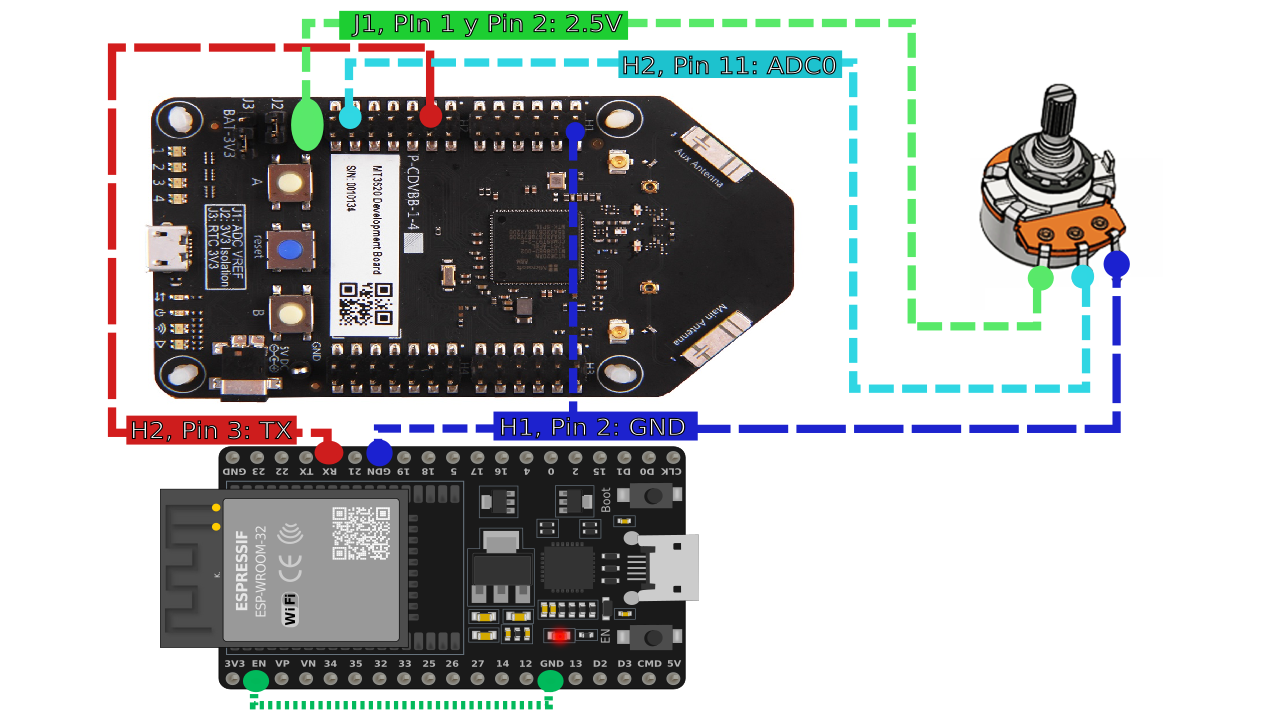
\includegraphics[scale=.40]{DiagramaDeConexion}
	\caption{Diagrama de conexiones.}
\end{figure}
\linebreak
El potenciómetro hará que varié la lectura del ADC. El ESP32 se está usando como un UART a USB, lo necesitas conectar a una computadora y leerlo en una terminal serial. Este nos dará los mensajes que envié el MT3620. El ESP32 se puede reemplazar por adaptadores UART a USB si se desea.
\pagebreak
\subsection{Códigos}
\label{sec:codigos}
\begin{itemize}
	\item 
	\href{https://github.com/Javier20060904/ejemplo_HL}{ejemplo\textunderscore HL}: Este programa consiste en el uso de ADC, GPIO y UART usando las API's de Azure Sphere en alto nivel.
	\item
	\href{https://github.com/Javier20060904/ejemplo_RT}{ejemplo\textunderscore RT}:  Este programa consiste en el uso de ADC, GPIO y UART usando los drivers de Mediatek junto al FreeRTOS.
	\item 
	\href{https://github.com/Azure/azure-sphere-samples/tree/main/Samples/AzureIoT}{Sample: Azure IoT}: Ejemplo proveído por Microsoft. Simula un termómetro y envía los datos de lectura a un IoT Hub.
\end{itemize}


